% !TEX encoding = UTF-8 Unicode
% !TEX root = ../main.tex
% !TEX spellcheck = en-US



% DEFINITION AND CHALLENGES, HOW IT RELATES TO THIS THESIS

% LINKING WORDS ARE IMPORTANT; similarly, in addition, also, again
% Disagreements; however, on the otehr hand, conversely, nevertheless

% Structure:

% - Introduction/definition of topic

\chapter{State-of-the-Art}
\label{chap:sota}

\textit{\textbf{Report Overview}}
\begin{itemize}
	\item \textit{1. Introduction}
	\item \textit{\textbf{2. State-of-the-Art}}
	\item \textit{3. Research Methodology}
	\item \textit{4. Results}
	\item \textit{5. Discussion}
	\item \textit{6. Conclusion}
\end{itemize} \


This chapter presents the relevant state-of-the-art for this thesis. Section 2.1 presents the metaphor of technical debt. 




%%%%%%%%%%%%%%%%%%%%%%%%%%%%%%%%%%%%%%%%%%%%%%% TECHNICAL DEBT %%%%%%%%%%%%%%%%%%%%%%%%%%%%%%%%%%%%%%%%%%%%%%%



\section{Technical Debt}
\label{sec:techdebt}
The metaphor of technical debt was first introduced by Ward Cunningham in 1992 to communicate technical problems with non-technical stakeholders\cite{p29-cunningham}. To deliver business functionality as quick as possible, \textit{'quick and dirty'} decisions are often made. These decisions may have short-term value, but it could affect future development and maintenance activities negatively. Cunningham was the first one who drew the comparison between technical complexity and financial debt in a 1992 experience report\cite{p29-cunningham}: 

\begin{displayquote}
	\textit{“Shipping first time code is like going into debt. A little debt speeds up the development as long as it is paid back promptly with a rewrite... The danger occurs when the debt is not repaid. Every minute spent on not-quite-right code counts as interest on that debt. Entire engineering organizations can be brought to a stand-still under the debt load of an unconsolidated implementation, object-oriented or otherwise.” - Ward Cunningham, 1992}.
\end{displayquote}

The concept refers to the financial world where going into debt means repaying the loan with interest\cite{p50-allman}. Like financial debt, technical debt accrues interest over time. Interest is defined as the extra effort that has to be dedicated in the future development in order to modify the part of the software that contains technical debt\cite{p31-guo,p35-klinger,li2015systematic}. Unmanaged technical debt can cause projects to face significant technical and financial problems, which ultimately leads to increased maintenance and evolution costs\cite{nord2012search}. 



\subsection{Definitions of Technical Debt}
Several researchers have attempted to give us a clear picture of what technical debt is\cite{url-fowler,url-mcconnell,krutchen}. Fowler\cite{url-fowler} presents a technical debt quadrant which consists of two dimensions: \textit{reckless/prudent} and \textit{deliberate/inadvertent}\cite{url-fowler}. Technical debt quadrant in Figure \ref{fig:techDebtQuad} indicates four types of technical debt: \textit{reckless/deliberate}, \textit{reckless/inadvertent}, \textit{prudent/deliberate}, and \textit{prudent/inadvertent}. Reckless/Deliberate debt is usually incurred when technical decisions are taken intentionally without any plans on how to address the problem in the future. A team may know about good design practices, but still implements \textit{'quick and dirty'} solutions because they think they cannot afford the time required to write clean code. The second type is reckless/inadvertent. It is incurred when best practices for code and design are being ignored, ultimately leading to a big mess of spaghetti code. Prudent/Deliberate debt occurs when the value of implementing a ‘quick and dirty’ solution is worth the cost of incurring the debt to meet a short-term goal. The team is fully aware of the consequences, and have a plan on how to address the problem in the future. At last, we have prudent/inadvertent debt. This type of debt occurs when a team realizes that the design of a valuable software could have been better after delivering it. A software development process is as much as learning as it is coding.

\begin{figure}[ht!]
	\centering
	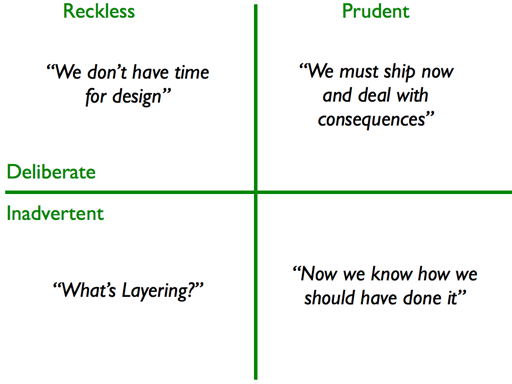
\includegraphics[width=0.8\textwidth]{images/techDebtQuadrant.png}
	\caption{Fowler's Technical Debt Quadrant}
	\label{fig:techDebtQuad}
\end{figure}

McConnell\cite{url-mcconnell} classified technical debt as intentional and unintentional debt. Intentional debt is described as debt that is incurred deliberately. For example, an organization makes a strategic decision that aims to reach a certain objective by taking a shortcut they are fully aware of. Intentional debt can further be viewed as short-term and long-term debt\cite{p8-codabux,mcconnel-slides}. Short-term debt is usually incurred reactively, for tactical reasons. Long-term debt is usually incurred pro-actively, for strategic reasons. Unintentional debt is described as debt that is incurred inadvertently due to lack of knowledge or experience. For example, a junior software developer may write low quality code that does not conform with standard coding standard due to low experience. 

Krutchen et al.\cite{krutchen} presented a technical debt landscape for organizing technical debt. They distinguished visible elements such as new functionality to add or defects to fix, and the invisible elements that are only visible to software developers. On the left side of Figure \ref{fig:techDebtLandscape}, technical debt affects evolvability of the system, while on the right side, technical debt mainly affects software maintainability. 

\begin{figure}[ht!]
	\centering
	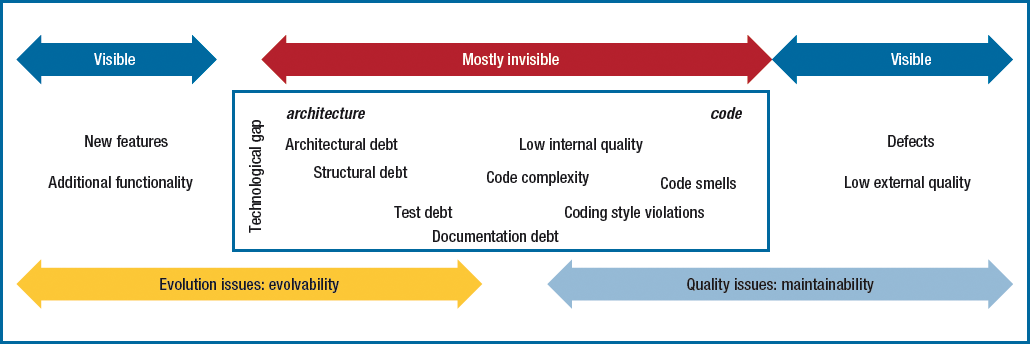
\includegraphics[width=1.0\textwidth]{images/techDebtLandscape.png}
	\caption{Technical Debt Landscape}
	\label{fig:techDebtLandscape}
\end{figure}

\subsection{Classification of Technical Debt}
\label{sub:classificationtechdebt}
Technical debt can accumulate in many different ways, and therefore it is important to distinguish the various types of technical debt. Multiple studies\cite{li2015systematic,p8-codabux,foser076-brown,tom2013exploration,Zazworka:2011:PDD:1985362.1985372,Zazworka:2013:CSE:2460999.2461005} have pointed out several subcategories of technical debt based on its association with traditional software life-cycle phases; architectural debt, code debt, defect debt, design debt, documentation debt, infrastructure debt, requirements debt, and test debt. Table \ref{tab:subcategories} lists the different subcategories of technical debt.

\begin{table}
	\resizebox{\textwidth}{!}{
	\centering
	\begin{tabular}{ | p{5cm} | p{8cm} |}
	\hline
	\textbf{Subcategory} & \textbf{Definition} \\ \hline
	Architectural debt\cite{li2015systematic,p8-codabux,foser076-brown} & Architectural decisions that make compromises in some of the quality attributes, such as modifiability. \\ \hline
	Code debt\cite{li2015systematic,foser076-brown,tom2013exploration} & Poorly written code that violates best coding practices and guidelines, such as code duplication. \\ \hline
	Defect debt\cite{li2015systematic,tom2013exploration} & Defect, failures, or bugs in the software. \\ \hline
	\textbf{Design debt}\cite{li2015systematic,Zazworka:2011:PDD:1985362.1985372,foser076-brown} & \textbf{Technical shortcuts that are taken in design}.\\ \hline
	Documentation debt\cite{li2015systematic,foser076-brown,Zazworka:2013:CSE:2460999.2461005} & Refers to insufficient, incomplete, or outdated documentation in any aspect of software development.\\ \hline
	Infrastructure debt\cite{li2015systematic,tom2013exploration,p8-codabux} & Refers to sub-optimal configuration of development-related processes, technologies, and supporting tools. An example is lack of continuous integration.\\ \hline
	Requirements debt\cite{li2015systematic,Zazworka:2013:CSE:2460999.2461005} & Refers to the requirements that are not fully implemented, or the distance between actual requirements and implemented requirements.\\ \hline
	Test debt\cite{li2015systematic,Zazworka:2013:CSE:2460999.2461005,foser076-brown} & Refers to shortcuts taken in testing. An example is lack of unit tests, and integration tests.\\
	\hline
	\end{tabular}}
	\caption{Types of Technical Debt} \label{tab:subcategories}
\end{table}


\subsection{Causes and Effects of Technical Debt}
Several researchers have investigated the reasons to incur technical debt. Klinger et al.\cite{p35-klinger} conducted an industrial case study at IBM where four technical architects with different backgrounds were interviewed. The goal was to examine how decisions to incur debt were taken, and the extent to which the debt provided leverage\cite{p35-klinger}. The study revealed that the company failed to assess the impact of intentionally incurring debt on projects. Decisions regarding technical debt were rarely quantified. The study also revealed big organizational gaps among the business, operational, and technical stakeholders. When the project team felt pressure from the different stakeholders, technical debt decisions were made without quantifications of possible impacts.

Lim et al.\cite{lim-taksande} pointed out that technical debt is not always the result of poor developer disciplines, or sloppy programming. It can also include intentional decisions to trade off competing concerns during business pressure. Furthermore, Li et al. explains that technical debt can be used in short term to capture market share and to collect customers feedback early. In the long term, technical debt tended to be negative. These trade-offs included increased complexity, reduced performance, low maintainability, and fragile code. This led to bad customer satisfaction and extra working hours. In many cases, the short term benefits of technical debt outweighed the future costs.

Guo et al.\cite{guo2011tracking} studied the effects of technical debt by tracking a single delayed maintenance task in a real software project throughout its life-cycle, and simulated how managing technical debt can impact the project result. The results indicated that delaying the maintenance task would have almost tripled the costs, if it had been done later.

Siebra et al.\cite{p247-siebra} carried out an industrial case study where they analyzed documents, emails, and code files. Additionally, they interviewed multiple developers and project managers. The case study revealed that technical debt were mainly taken by strategic decisions. Furthermore, they commented out that using a unique specialist could lead the development team to solutions that the specialist wanted and believe were correct, leading the team to incur debt. The study also identified that technical debt can both increase and decrease the amount of working hours.

Zazworka et al.\cite{zazworka2011investigating} studied the effects of \textit{God Class} code smell and technical debt on software quality. \textit{God Class} are examples on bad coding, and therefore includes a possibility for refactoring\cite{Zazworka:2011:PDD:1985362.1985372}. The results indicated that \textit{God Class} code smell requires more maintenance effort including bug fixing and changes to software that are considered as a cost to software project. In other words, if developers desire higher software quality, then technical debt needs to be addressed closely in the development process.

Buschmann\cite{buschmann2011pay} explained three different stories of technical debt effects. In the first case, technical debt accumulated in a platform started had growth to a point where development, testing, and maintenance costs started to increase dramatically. Additionally, the components were hardly usable. In the second case, developers started to use shortcuts to increase the development speed. This resulted in significant performance issues because an improper software modularization reflected organizational structures instead of the system domains. It ended up turning into economic consequences. In the last case, an existing software product experienced increased maintenance cost due to architectural erosion. However, management analyzed that re-engineering the whole software would cost more than doing nothing. Management decided not to do anything to technical debt, because it was cheaper from a business point-of-view.

Codabux et al.\cite{p8-codabux} carried out an industrial case study where the topic was agile development focusing on technical debt. They observed and interviewed developers to understand how technical debt is characterized, addressed, prioritized, and how decisions led to technical debt. Two subcategories of technical debt were commonly described in this case study; infrastructure and automation debt. 

These studies indicates that the causes and effects of technical debt are not always caused by technical reasons. Technical debt can be the result of intentional decisions made by the different stakeholders. Incurring technical debt may have short-term positive effects such as time-to-market benefits. Not paying down technical debt can result economic consequences, or quality issues in the long-run. The allowance of technical debt can facilitate product development for a period, but decreases the product maintainability in the long-term. However, there are some times where short-term benefits overweight long-term costs\cite{guo2011tracking}. 


\subsection{Identification of Technical Debt}
Technical debt accumulation may cause increased maintenance and evolution costs. At worst, it may even cancel out projects. The first step towards managing technical debt is to properly identify and visualize  technical debt items. 

According to Zazworka et al.\cite{zazworka2014comparing}, there are four main techniques for identifying technical debt in source code: modularity violations, design patterns and grime buildup, code smells, and automatic static analysis issues. 

\subsubsection{Modularity Violation}
Software modularity determines software quality in terms of evolveability, changeability, and maintainability\cite{huynh2007evolutionary}, and the essence is to allow modules to evolve independently. However, in reality, two software components may change together though belonging to distinct modules, due to unwanted side effects caused by \textit{'quick and dirty'} solutions\cite{wong2011detecting,zazworka2014comparing}. This causes a violation in the software designed modular structure, which is called a modularity violation. Wong et al.\cite{wong2011detecting} identified 231 modularity violations from 490 modification requests in their experiment using Hadoop. 152 of the 490 identified violations were confirmed by the fact that they were either addressed in later versions of Hadoop, or recognized as problems by the developers. In addition, they identified 399 modularity violation from 3458 modification request of Eclipse JDT\cite{wong2011detecting}. Among these violations, 161 were confirmed. Zazworka et al.\cite{zazworka2014comparing} revealed that the average number of modularity violations per class in release 0.2.0 to release 0.14.0 of Hadoop ranged from 0.04 to 0.11. They identified 8 modularity violations in the first release of Hadoop and 37 in the last one. In addition, they revealed that modularity violations are strongly related to classes with high defect- and change-proneness. 



\subsubsection{Design Pattern and Grime Buildup}
Patterns are known to be general solutions to recurrent design problems. They are commonly used to improve maintainability, flexibility, and architecture design of software systems by reducing the number of defects and faults. Twenty-three design patterns are widely used in software development and is classified into three types\cite{Desig53:online}: \textit{creational}, \textit{behavioral}, and \textit{structural}. Creational design patterns are all about class instantiation. This pattern can be divided into class-creation patterns and object-creational patterns. Creational patterns include patterns such as Abstract Factory, Builder, Factory Method, Object Pool, Prototype, and Singleton\cite{Desig53:online}. Structural design patterns are all about Class and Object composition. They include patterns such as Adapter, Bridge, Composite, Decorator, Facade, Flyweight, Private Class Data, and Proxy\cite{Desig53:online}. Lastly, behavioral design patterns are all about class's objects communication, and are concerned with communication between objects. Behavioral patterns include patterns such as Chain of Responsibility, Command, Interpreter, Iterator, Mediator, Memento, Null Object, Observer, State, Strategy, Template Method, and Visitor\cite{Desig53:online}. 

Software continuously evolve in response to external demands for new functionality. One consequence of such evolution is software design decay. Izurieta et al.\cite{izurieta2007software} defines decay the deterioration of the internal structure of system designs. Furthermore, they define design pattern decay as deterioration of the structural integrity of a design pattern realization. As a pattern realization evolves, its structure and behavior tend to deviate from its original intent. Changes in the code base could lead to code ending up outside the pattern. This is known as design grime, non-pattern related code\cite{izurieta2007software}. Moreover, design patterns can also rot, when changes break the structural and functional integrity of a pattern\cite{izurieta2007software}. Izurieta et al.\cite{izurieta2013multiple} examined the extent to which software designs actually decay, rot, and accumulate grime in three open-source systems. They found no evidence of design patterns rot, but they found evidence of pattern decay due to grime. Furthermore, Izurieta et al.\cite{izurieta2008testing} also studied the consequences of grime buildup on testability of general purpose design patterns. Their result reveals that as systems age, the growth of grime and the appearance of anti-patterns increase testing requirements.



\subsubsection{Code Smell}
\label{subsub:codesmell}
Some forms of technical debt accumulate over time in the form of source code\cite{zazworka2014comparing}. Fowler et al.\cite{fowler1999refactoring} describes the concept of code smells as choices in object-oriented systems that do not comply with the principles of good object-oriented design and programming practices. They are an indication of that some parts of the design is inappropriate and that it can be improved. Code smells are usually removed by performing one or more refactoring\cite{fowler1999refactoring}. For instance, one such smell is "Long Method", a method with too many lines of code. This type of code smell can be refactored by 'Extract Method', by reducing the length of the method body\cite{fowler1999refactoring}. 

Mäntylä et al.\cite{mantyla2003taxonomy} proposes a taxonomy based on the criteria on code smells defined by Fowler et al.\cite{fowler1999refactoring}. The taxonomy categories code smells into seven groups of problems: bloaters, object-oriented abusers, change preventers, dispensables, encapsulators, couplers, and others. The first class, Bloaters, represents large pieces of code that cannot be effectively handled. Object-oriented abusers are related to cases where the solution does not exploit the the possibilities of object-oriented design. Change preventers refers to code structure that considerably hinder the modification of software. Dispensables represent code structure with no value. Encapsulators deal with data communication mechanism or encapsulation. Couplers refer to classes with high coupling. The last group of problem is Other, which refers to code smells that do not fit into any of the other categories. This includes \textit{Incomplete Library Class} and \textit{Comments}. Table \ref{tab:codesmell} lists all the code smells that are presented by Fowler et al.\cite{fowler1999refactoring}.


\begin{table}[]
\centering
\caption{Code Smell Taxonomy}
\label{tab:codesmell}
\begin{tabular}{|l|l|}
\hline
\textbf{Code Smell}                           & \textbf{Group}    \\ \hline
Long Method                                   & Bloaters          \\ \hline
Large Class                                   & Bloaters          \\ \hline
Primitive Obsession                           & Bloaters          \\ \hline
Long Parameter List                           & Bloaters          \\ \hline
Data Clumps                                   & Bloaters          \\ \hline
Switch Statements                             & O-O Abusers       \\ \hline
Temporary Field                               & O-O Abusers       \\ \hline
Refused Bequest                               & O-O Abusers       \\ \hline
Alternative Classes with Different Interfaces & O-O Abusers       \\ \hline
Parallel Inheritance Hierarchies              & O-O Abusers       \\ \hline
Divergent Change                              & Change Preventers \\ \hline
Shotgun Surgery                               & Change Preventers \\ \hline
Lazy Class                                    & Dispensables      \\ \hline
Data Class                                    & Dispensables      \\ \hline
Duplicated Code                               & Dispensables      \\ \hline
Speculative Generality                        & Dispensables      \\ \hline
Message Chains                                & Encapsulators     \\ \hline
Middle Man                                    & Encapsulators     \\ \hline
Feature Envy                                  & Couplers          \\ \hline
Inappropriate Intimacy                        & Couplers          \\ \hline
Comments                                      & Other             \\ \hline
Incomplete Library Class                      & Other             \\ \hline
\end{tabular}
\end{table}

Several studies have been conducted to investigate the relationship between code smell and change-proneness of classes in object-oriented source code. A study by Olbrich et al.\cite{olbrich2009evolution} revealed that different phases during evolution of code smells could be identified, and classes infected with code smells have a higher change frequency; such classes seem to need more maintenance than non-infected classes. Khomh et al.\cite{khomh2009exploratory} investigate if classes with code smells are more change-prone than classes without smells. After studying 9 releases of Azureus and 13 releases of Eclispe, their findings show that classes with code smells are more change-prone than others.

Multiple approaches have been proposed for identifying code smells, ranging from manual approaches to automatic. Manual detection of code smells can be done by code inspections\cite{travassos1999detecting}. Travassos et al.\cite{travassos1999detecting} present a set of reading techniques that gives specific and practical guidance for identifying defects in Object-Oriented design. However, Marinescu\cite{marinescu2001detecting} argue that manual code inspection can be time expensive, unrepeatable, and non-scalable. In addition, it is often unclear what exactly to search for when inspecting code\cite{ciupke1999automatic}. Moreover, a study by Mäntylä revealed more issues regarding manual inspection of code. He states that manual code inspection is hard due to conflicting perceptions of code smells among the developers, causing a lack of uniformity in the smell evaluation. 

Automatic approaches for identifying code smells reduce the effort of browsing through large amounts of code during code inspection process. Ciupke\cite{ciupke1999automatic} propose an approach for detecting code smells in object-oriented systems. In this approach, code smells to be identified are specified as queries. The result of a queries is a piece of design specifying the location of the code smell in the source code. This approach was applied to several case studies, both in academical and industrial context. Their findings revealed that code smell detection can be automated to a large degree, and that the technique can be effectively applied to real-world code.

Another method for automatic detection of code smells is done by using metrics. Marinescu\cite{marinescu2001detecting} propose a general metric-based approach to identify code smells. Instead of a purely manual approach, the use code metrics were proposed for detecting design flaws in object-oriented systems. This approach were later refined, with the introduction of detection strategies\cite{marinescu2004detection}. Based on their case study, the precision of automatic detection of code smells is reported to be 70\%. Furthermore, a study by Schumacher et al.\cite{schumacher2010building} investigated how human elicitation of technical debt by detecting god class code smells compares to automatic approaches by using a detection strategy for god classes. Their findings show that humans are able to detect code smells in an effective way if provided with a suitable process. Moreover, the the findings revealed that the automatic approach yield high recall and precision in this context. 

%%Other researchers designed visualization for inspecting code smells. Parnin et al. introduced a Visual Studio plugin which allows the developers to search for various code smells in source code.


\subsubsection{Automatic Static Analysis Issues}
The identification of software design and code issues can be done with automatic static analysis code tools. Automatic static analysis tools looks for violations of recommend programming practices on source code line level that might cause faults or degrade some parts of software quality\cite{zazworka2014comparing}. Tools are able to alert software developers of potential problems in the source code, and they may suggest refactoring solutions to avoid future problems. Several tools for detecting code and design issues have been proposed in the literature\cite{rutar2004comparison}. These tools have been applied by several researchers\cite{zazworka2014comparing,copeland2005pmd,codabux2016technical,rutar2004comparison}, and the overall finding is that a small set of automatic static analysis issues are related to defects in the software. However, the set of issues depends on the context and type of software analyzed. Despite the fact that a tool indicates a potential problem in the source code, it takes human judgment to determine if something could be problematic down the road. 



\subsection{Strategies and Practices for Managing Technical Debt}
Managing technical debt compromises the actions of identifying the debt and making decisions about which debt that should be repaid\cite{fowler1999refactoring,krutchen,Zazworka:2011:PDD:1985362.1985372}. There are three high-level steps that are required to manage technical debt\cite{suryanarayana2014refactoring}: \textit{Increasing awareness of technical debt}, \textit{detecting and repaying technical debt}, and \textit{prevent accumulation of technical debt}. \textit{Increasing awareness of technical debt} is the first step towards technical debt management. This includes awareness of the concept of technical debt, its different forms, the impact of technical debt, and the factors that contribute to technical debt. Awareness will help an organization taking the right decisions to achieve their goals. The second step is \textit{detecting and repaying technical debt}. This step is focused on determining the extent of technical debt in the software. Identifying specific instances of debt and their impact can help us to prepare a plan to recover from the debt. The final step, \textit{prevent accumulation of technical debt}, ensures that technical debt does not increase and remains manageable in the future. Best practices such as refactoring, re-engineering, and testing is necessary to manage the debt\cite{p8-codabux}. This step also involves collaboration between all stakeholders to collectively track and monitor the debt. For example, using a backlog during release and iteration planning to list debt-related tasks\cite{krutchen}. Guo et al.\cite{p31-guo} suggest using a portfolio for technical debt management. This approach collects technical debt items to a \textit{"Technical Debt List"}, which may potentially be used to pay technical debt based on its cost and value. Tools may also be used for technical debt management. SonarQube is an open source application for quality management\cite{sonarsource2013sonarqube}. It can assess the debt in a software project by performing automatic static code analysis. Each automatic static analysis issue is assigned a score based on how much work it requires to fix that error. The analysis gives the total sum of technical debt for the entire product.







%%%%%%%%%%%%%%%%%%%%%%%%%%%%%%%%%%%%%%%%%%%%%%% DESIGN TECHNICAL DEBT %%%%%%%%%%%%%%%%%%%%%%%%%%%%%%%%%%%%%%%%%%%%%%%


\section{Design Debt}
\label{sec:designdebt}
Design debt is one of the instances of technical debt\cite{li2015systematic,Zazworka:2011:PDD:1985362.1985372,foser076-brown}. It is concerned with the design aspects of technical debt. Design debt includes design smells and violations of design rules. Design smells are certain structures in the design that indicate violation of fundamental design principles and negatively impact design quality\cite{suryanarayana2014refactoring}. A possible symptom of design debt is when code structures drift away from good object-oriented design principles\cite{zazworka2011investigating}. There are various reasons for software projects to run into design debt. For example, a common object-oriented design principle tells that a class should have a single purpose and should not implement many functions of the system. A class that tries to accomplish too many purposes is known as \textit{God Class} code smell. As we have mentioned earlier, code smells are an example design flaws in object-oriented design, which may potentially lead to maintainability issues in future evolution of the software system\cite{olbrich2009evolution}.

Suryanarayana et al.\cite{suryanarayana2014refactoring} present six common causes of design debt: \textit{violation of design principles}, \textit{inappropriate use of patterns}, \textit{language limitations}, \textit{procedural thinking in object-oriented paradigm}, \textit{viscosity}, and \textit{non-adherence to best practices and processes}. Design principles provide guidance to designers in creating high quality software. \textit{Violation of design principles} are manifested as smells. For example, code smells are symptoms of design violations in the source code. \textit{Inappropriate use of patterns} is related to the use of patterns without fully understanding the context, and the finer aspects and implications of using a particular variation of a pattern which. In some cases, misuse of a design pattern may potentially lead to an antipattern. \textit{Language limitations} is related to deficiencies in programming languages. \textit{Procedural thinking in object-oriented paradigm} is related to using procedural programming techniques in object-oriented paradigm. For example, using imperative names for classes, functional decomposition, and missing polymorphism with explicit type checks results in design smells in an object-oriented context. \textit{Viscosity} is one of the reasons to use hacks instead of adopting a systematic process to achieve a particular requirement. Lastly, \textit{Non-adherence to practices and processes} is related to best practices and processes that are not followed correctly or completely. 




%%%%%%%%%%%%%%%%%%%%%%%%%%%%%%%%%%%%%%%%%%%%%%% SOFTWARE QUALITY %%%%%%%%%%%%%%%%%%%%%%%%%%%%%%%%%%%%%%%%%%%%%%%

\section{Software Quality}
\label{sec:softwarequality}
According to the IEEE Standard Glossary of Software Engineering Terminology\cite{radatz1990ieee}, the quality of a software is defined as \textit{1) the degree to which a system, component, or process meets specified requirements}, and \textit{2) the degree to which a system, component, or process meets customer or user needs or expectations}. ISO/IEC 9126:2001 offer a valuable conceptual framework for software quality, where a distinction between \textit{quality in use}, \textit{external quality}, and \textit{internal quality} is made\cite{ISOIEC9126}. \textit{Quality in use} refers to the users view of system quality. \textit{External quality} reflects the dynamic aspect of a software application, and is subdivided into six quality attributes. \textit{Internal quality} refers to the criteria of each quality attribute. Software quality can be measured by using a product quality model. ISO/IEC 9126:2001 classifies software quality in a structured set of six quality attributes\cite{ISOIEC9126}. Bass et al.\cite{Bass:2012:SAP:2392670} describes these characteristics as software quality attributes. Table \ref{tab:qaAttributes} present the ISO/IEC 9126:2001 quality model, with the quality attributes, and their criteria.  

\begin{table}[ht!]
	\resizebox{\textwidth}{!}{
	\centering
	\caption{Software quality attributes, criteria, and description (ISO/IEC 9126)}
	\label{tab:qaAttributes}
    \begin{tabular}{|l|p{3cm}|p{5cm}|} 
    \hline
    \textbf{Quality Attribute} & \textbf{Criteria}             & \textbf{Description} \\ \hline 
    Functionality      & ~                    & Systems ability to do work for which it was intended.          \\ \hline
    ~                  & Suitability          & ~           \\ \hline
    ~                  & Accuracy             & ~           \\ \hline
    ~                  & Interoperability     & ~           \\ \hline
    ~                  & Security             & ~           \\ \hline
    ~                  & Compliance       	  & ~           \\ \hline
    Reliability        & ~                    & Systems ability to keep operating over time under certain conditions.           \\ \hline
    ~                  & Maturity             & ~           \\ \hline
    ~                  & Fault Tolerance      & ~           \\ \hline
    ~                  & Recoverability       & ~           \\ \hline
    ~                  & Compliance       	  & ~           \\ \hline
    Usability          & ~                    & Systems ability to be understood, learned, and used by others.           \\ \hline
    ~                  & Understandability    & ~           \\ \hline
    ~                  & Learnability         & ~           \\ \hline
    ~                  & Operability          & ~           \\ \hline
    ~                  & Attractiveness       & ~           \\ \hline
    ~                  & Compliance       	  & ~           \\ \hline
    Efficiency         & ~                    & Systems ability to provide appropriate performance relative to the amount of resources used under stated conditions.          \\ \hline
    ~                  & Time behaviour       & ~           \\ \hline
    ~                  & Resource utilization & ~           \\ \hline
    ~                  & Compliance       	  & ~           \\ \hline
    Maintainability    & ~                    & Systems ability to be modified in the future.           \\ \hline
    ~                  & Analyzeability       & ~           \\ \hline
    ~                  & Changeability        & ~           \\ \hline
    ~                  & Stability            & ~           \\ \hline
    ~                  & Testability          & ~           \\ \hline
    ~                  & Compliance       	  & ~           \\ \hline
    Portability        & ~                    & Systems ability to be transferred from one environment to another.          \\ \hline
    ~                  & Adaptability         & ~           \\ \hline
    ~                  & Installability       & ~           \\ \hline
    ~                  & Co-existence         & ~           \\ \hline
    ~                  & Replaceability       & ~           \\ \hline
    ~                  & Compliance       	  & ~           \\ \hline
    
    \end{tabular}}
\end{table}



\section{Object-Oriented Metrics}
\label{sec:oometrics}
Object-Oriented metrics have been proposed as a quality indicator for object-oriented software systems. There are three traditional metrics that are widely used, and are well understood by researchers and practitioners\cite{quenelobject}. These metrics are: \textit{cyclomatic complexity}, \textit{size}, and \textit{comment percentage}. \textit{Cyclomatic complexity} evaluates the complexity of an algorithm in a method. It is recommended that the \textit{cyclomatic complexity} for a method should be below 10\cite{quenelobject}. \textit{Size} of a method is used evaluate the understandability of the code. \textit{Size} is measured in many different ways, including all physical lines of code, lines of statements, and number of blank lines. \textit{Comment percentage} measures the number of comments in percent by counting total number of comments divided on total lines of code minus number of blank lines.

Chidamber and Kemerer\cite{chidamber1994metrics} proposed a set of six software metrics to identify certain design traits of a software component. These metrics are: \textit{Weighted Methods per Class (WMC), Depth of Inheritance Tree (DIT), Number of Children (NOC), Lack of Cohesion in Methods (LCOM), Coupling Between Objects (CBO), and Response For a Class (RFC)}. The \textit{WMC} is used to count the number of methods in a class, or to count the of sum of complexities of all methods in a class. The complexity of a method is measured by \textit{cyclomatic complexity}. This metric measures understandability, maintainability, and reusability\cite{quenelobject}. The \textit{DIT} metric measure the maximum number of steps from a class node to the root in the inheritance hierarchy. The deeper a class is withing the hierarchy, the greater number of methods it is likely to inherit, making it more complex to predict its behavior\cite{quenelobject}. Moreover, this metric are related to efficiency, reusability, understandability, and testability\cite{quenelobject}. \textit{NOC} metric measures the number of subclasses of a class in a hierarchy. The greater number of children may be an indication of subclasses misuse or improper parent abstraction. This metric evaluates efficiency, reusability, and testability\cite{quenelobject}. The \textit{LCOM} is used to measure the lack of cohesion in methods of a class. It measures the dissimilarity of methods in a class by looking at the instance variables or attributes used by the methods. High cohesion indicates good subdivision, while low cohesion increase the complexity of a class. This metric measures efficiency and reusability\cite{quenelobject}. The \textit{CBO} metric counts the number of other classes to which a class is coupled. Excessive coupling is detrimental to modular design and prevents reuse\cite{quenelobject}. Larger number of coupled objects indicates higher sensitivity to changes in other parts of the design. \textit{CBO} evaluates efficiency and reusability\cite{quenelobject}. The \textit{RFC} metric counts the total number of methods in a class that can be invoked in a response to a message sent to an object. This metric includes all methods accessible within the class hierarchy. \textit{RFC} metric evaluates understandability, maintainability, and testability\cite{quenelobject}. Basili et al.\cite{basili1996validation} investigated Chidamber and Kemerer's suite of metrics. Their result claim that several of Chidamber and Kemerer's object-oriented metrics appear to be useful to predict fault-prone classes during early phases of the software life-cycle. Similarly, Li et al.\cite{li1993object} conclude that object-oriented metrics are able to predict maintenance effort.




%%%%%%%%%%%%%%%%%%%%%%%%%%%%%%%%%%%%%%%%%%%%%%% SOFTWARE MAINTENANCE AND EVOLUTION %%%%%%%%%%%%%%%%%%%%%%%%%%%%%%%%%%%%%%%%%%%%%%%


\section{Software Evolution and Maintenance}
\label{sec:maintenance}
Increasingly, more and more software developers are employed to maintain and evolve existing systems instead of developing new systems from scratch\cite{Sommerville:2011:SE}. Lehman\cite{lehman1980programs} introduced the study of software evolution. Software evolution is a process that usually takes place when the initial development of a software project is done and was successful\cite{Bennett:2000:SME:336512.336534}. The goal of software evolution is to incorporate new user requirements in the application, and adapt it to the existing application. Software evolution is important because it takes up to 85-90\% of organizational software costs\cite{Sommerville:2011:SE}. In addition, software evolution is important because technology tend to change rapidly.

Software maintenance is defined as \textit{modifications of a software after delivery to correct faults, ti improve performance or other attributes, or to adapt the product to a modified environment}\cite{720567}. Maintenance can be classified into four types\cite{Bennett:2000:SME:336512.336534,720567}: \textit{adaptive maintenance}, \textit{perfective maintenance}, \textit{corrective maintenance}, and \textit{preventive maintenance}. \textit{Adaptive maintenance} is the modification of a software product performed after delivery to keep the computer program usable in a changed or changing environment. \textit{Perfective maintenance} is the modification of a software product after delivery to improve performance and maintainability. \textit{Corrective maintenance} is the reactive modification of a software product performed after delivery to correct discovered faults. Lastly, \textit{Preventive maintenance} is the maintenance performed for the purpose of preventing problems before they occur.

Van Vliet\cite{Vliet:2008:SEP:1481475} states that the real maintenance activity is corrective maintenance. 50\% of the total software maintenance is spent on perfective, 25\% on adaptive maintenance, and 4\% on preventive maintenance. This leads to that 21\% of the total maintenance activity is corrective maintenance, the 'real' maintenance\cite{Vliet:2008:SEP:1481475}. This has not changed since the 1980s when Lientz and and Swanson conducted a study on software maintenance\cite{lientz1980software}. The study points out that most severe maintenance problems were caused by poor documentation, demands from users for changes, poor meeting scheduled, and problems training new hires.



%%%%%%%%%%%%%%%%%%%%%%%%%%%%%%%%%%%%%%%%%%%%%%% SOFTWARE REUSE %%%%%%%%%%%%%%%%%%%%%%%%%%%%%%%%%%%%%%%%%%%%%%%

\section{Software Reuse}
\label{sec:reuse}
Software reuse is the process of creating software systems from existing software rather than building software systems from scratch\cite{krueger1992software,frakes1996software}. There are many various techniques that can be used to achieve software reuse: \textit{abstraction}, \textit{compositional reuse}, \textit{generative reuse}, and \textit{generation vs. composition}\cite{sametinger1997software}. \textit{Compositional reuse} is based on the idea of reusable components. It supports bottom-up development of systems where low-level components are available. \textit{Compositional reuse} is also known as ad-hoc reuse or individual reuse. \textit{Generative reuse} is based on the reuse of a generation process. It is often domain-specific, and is concerned with artifacts such as requirements, designs, and subsystems\cite{frakes1994systematic}. \textit{Generative reuse} is also known as systematic reuse\cite{frakes1994systematic}. \textit{Generation vs. composition} is a combined approach. 

There are several "assets" from a software project that can be reused, including \textit{architectures, source code, data, designs, documentation, estimates, human interfaces, plans, requirements}, and \textit{test cases}\cite{frakes1996software}.

The most common benefits of software reuse are quality improvement and effort reduction. Software reuse includes lower costs, shorter development time, higher quality of reusable components, and higher productivity\cite{Slyngstad:2006:ESD:1159733.1159770,lim1994effects}. The quality of the software increases every time an asset is reused, because errors are discovered more frequently, thus making it easier to keep the artifact more stable\cite{sametinger1997software}. However, software reuse may cause problems as well. A case study on selected feature from self-driving miniature car development revealed that reuse of legacy, third party, or open-source code, was one of the root causes of technical debt accumulation\cite{6974884}. Furthermore, Morisio et al.\cite{995420} identified three main causes of failures associated with software reuse: \textit{not introducing reuse-specific processes}, \textit{not modifying non-reuse processes}, and \textit{not considering human factors}. These causes were combined with lack of commitment by top management. Organizations attempting to implement generative reuse face both technical and non-technical problems\cite{frakes1994success}. Technical problems includes challenges with tools, standards and technology. Non-technical problems include the human factor, cultural issues, economical issues, and organizational issues. 




%%%%%%%%%%%%%%%%%%%%%%%%%%%%%%%%%%%%%%%%%%%%%%% REFACTORING %%%%%%%%%%%%%%%%%%%%%%%%%%%%%%%%%%%%%%%%%%%%%%%

\section{Refactoring}
\label{sec:refactoring}
Fowler defines refactoring as a process of changing the software system in such way that it does not alter the external behavior of the code yet improves its internal structure\cite{fowler1999refactoring}. Refactoring increases the code readability and maintainability by cleaning up code in a way such that changes of defects is reduced\cite{fowler1999refactoring}. Refactoring is an act of improving the design and quality of an existing system\cite{Vliet:2008:SEP:1481475}. It is believed that refactoring improves software quality and developer productivity by making it easier to understand and maintain software source code\cite{Kim:2012:FSR:2393596.2393655}. According to Opdyke\cite{opdyke1992refactoring}, refactoring can be categorized into low-level and high-level refactoring. Low-level refactoring is related to changing a program entity, such as renaming a member variable. High-level refactoring is usually a sequence of low-level refactorings, such as defining an abstract superclass. In addition, Opdyke presents twenty-six low-level refactorings and three high-level refactorings. Fowler et al.\cite{fowler1999refactoring} have summarized the work of Opdyke by cataloging his refactorings along with many other refactoring techniques that have been collected over the years. Refactoring can be applied to three types of software artifacts: \textit{programs, designs}, and \textit{software requirements}. \textit{Programs} include refactoring at source code or program level. For example, \textit{Extract Method}\cite{fowler1999refactoring} is a refactoring technique that can be applied at this level. \textit{Designs} include refactoring at design level, for example in the form of UML models. Design pattern is an example of an artifact at this level. Lastly, \textit{software requirements} include refactoring at the level of requirements specification. For example, decomposing requirements into a structure of viewpoints.


% SI NOE OM DEFECT OG REFACTOR CONFLICT, IKKE ALLTID DET LØNNER SEG

%Refactoring depends on the type of design defect found in the system has has a direct influence on the software maintenance cost\cite{("Siter: A quantitative investigaton of software metrics threshold values at acceptable risk level")

%%%%%%%%%%%%%%%%%%%%%%%%%%%%%%%%%%%%%%%%%%%%%%% EMBEDDED SYSTEMS %%%%%%%%%%%%%%%%%%%%%%%%%%%%%%%%%%%%%%%%%%%%%%%

\section{Embedded Systems}
\label{sec:embeddedsystems}
The \textit{IEEE Standard Glossary of Software Engineering Terminologies} define embedded system as \textit{a computer system that is part of a larger system and performs some of the requirements of that system; for example, a computer system used in aircraft or rapid transit system}\cite{radatz1990ieee}. Embedded systems are special-purpose computer systems designed to perform certain dedicated functions under certain constraints. According to Koopman\cite{koopman1999embedded}, there are four types of embedded systems: \textit{general computing}, \textit{control systems}, \textit{signal processing}, and \textit{communication and networking}. The various types of embedded systems share common requirements such as: \textit{real-time requirements}, \textit{resource consumption}, \textit{dependability}, and \textit{life-cycle properties}\cite{crnkovic2004component}. Embedded systems are supposed to be failure-free\cite{you2013reliability}, but these requirements may hinder embedded systems to deliver reliable service given a disturbance to its services\cite{patil2009embedded}. 

Software constitutes only one part in embedded systems. Embedded software is defined as software part of a larger system which performs some of the requirements of that system\cite{radatz1990ieee}. Developing embedded software has proven to be difficult\cite{ebert2009embedded,sherman2008quality}. Embedded software not only have to meet the functional requirements of "what", but also the non-functionality or "quality" requirements expected of them\cite{sherman2008quality}. Non-functional requirements have come to be referred to as software quality attributes. Ebert et al.\cite{ebert2009embedded} state that quality of software in embedded systems is difficult to measure. Most behaviors for embedded systems are related to run-time quality attributes, depending on the system domain. For instance, reliability and safety qualities are important in the automotive domain\cite{pretschner2007software}, while performance and reliability is important in mission critical systems\cite{trienekens2010quality}. Other quality attributes such as maintainability and usability, are often compromised in favor of run-time quality attributes.


\subsection{Safety-Critical Systems}
Safety-critical systems are those systems whose failure could result in loss of life, significant property damage, or damage to the environment\cite{knight2002safety}. These systems put a huge demand on software reliability, because a minor error in safety-critical software can produce failure of a complete system\cite{ebert2009embedded,trienekens2010quality,pretschner2007software}. Consider the role of safety-critical systems is often critical, the importance of managing software quality is therefore necessary to deliver software in a useful, safe, and reliable way. Given the lack of focus on non-functional requirements, the amount of technical debt in safety-critical systems grow continuously. Insufficient requirements and testing are two major cost drivers in embedded software development\cite{ebert2009embedded,graaf2003embedded}. 40\% of all software defects results from insufficient requirements, especially non-functional requirements[6,7,45]\cite{ebert2009embedded,graaf2003embedded,washizaki2007quality}. Testing code consumes up to 40\% of development resources. In addition, testing may potentially require 15-50\% of total project duration\cite{ebert2009embedded}.  

